\section{Analysis}
\label{sec:analysis}

\subsection{Property distributions}
Here we will look at the frequency distributions (histograms) comparing the characteristics of CPSBs, RPSBs an their control galaxies.

TODO: include a definition of the S\'ersic index \citep{1963BAAA....6...41S, 1968adga.book.....S}, its significance in this context: ellipticals vs. disks, and how it is measured. The surface brightness profile of a galaxy is generally a function of radius from the nucleus. The rate of change of brightness can be described by the S\'ersic function. Low values of SI ~1 relate to disc-like spiral galaxies, whereas higher SI values of 3 or more are measured in galaxies with compact bright nuclei, indicative of more evolved systems.  

We compare the distributions of CPSBs with that of the RPSB sample in terms of S\'ersic index, stellar mass, and redshift. These distributions are taken from the data in Tables \ref{tab:my-CPSBs} and \ref{tab:my-RPSBs}. The frequency distribution histograms are plotted in Figures \ref{fig:Sersic-plot}, \ref{fig:stellar-mass-plot} and \ref{fig:redshift-plot} respectively.

\begin{figure}
    \centering
    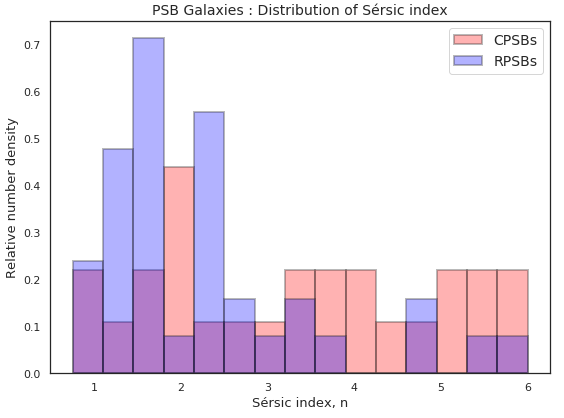
\includegraphics[width=\columnwidth]{images/JupyterPlots/Dist-Sersic-Index-All.png}
    \caption{Distribution of S\'ersic index (SI) values. The relative number density distribution of the S\'ersic index value for 26 CPSBs (red histogram) and 36 RPSBs (blue) are plotted. Those PSB galaxies with unreliable SI values (5) have been excluded. Generally CPSBs show higher SI values than RPBs. This indicates that CPBs tend to have concentrated nuclei contrary to the more disc-like RPSBs.}
    \label{fig:Sersic-plot}
\end{figure}

\begin{figure}
    \centering
    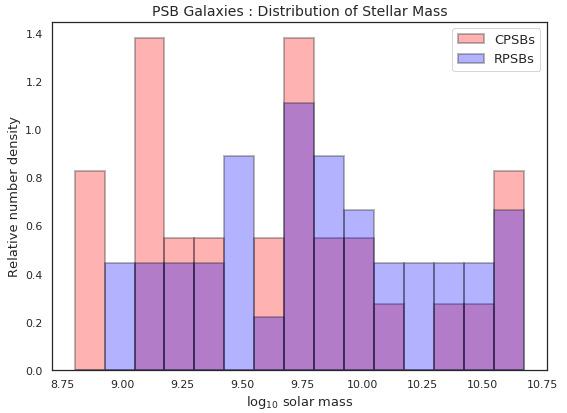
\includegraphics[width=\columnwidth]{images/JupyterPlots/Dist-Stellar-Mass-All.png}
    \caption{Distribution of Stellar mass of our sample of CPSBs (rad) and RPSBs (blue). On the scale of $\log_{10}$\Msun\ a fairly uniform distribution of stellar mass is apparent for both populations, CPSBs and RPSBs.}
    \label{fig:stellar-mass-plot}
\end{figure}

\begin{figure}
    \centering
    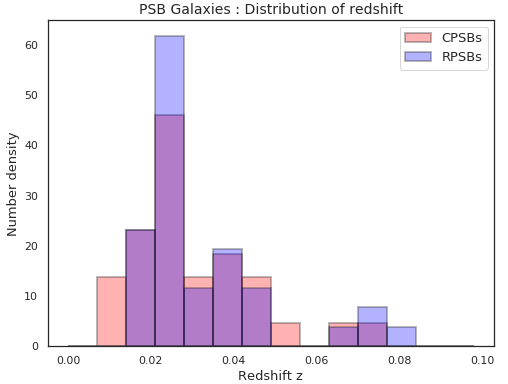
\includegraphics[width=\columnwidth]{images/JupyterPlots/Dist-z-All.png}
    \caption{Distribution in redshift. The redshift distribution of the CPSB sample is similar to that of the RPSB sample.}
    \label{fig:redshift-plot}
\end{figure}

\begin{figure}
    \centering
    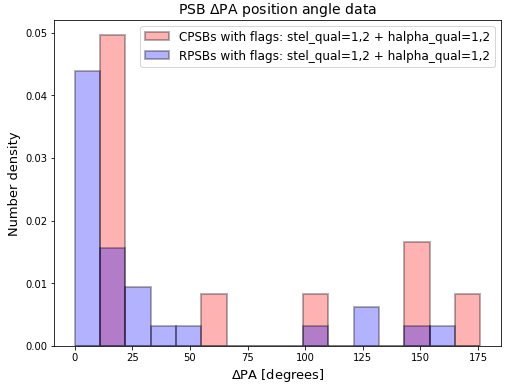
\includegraphics[width=\columnwidth]{images/JupyterPlots/Dist-Delta-PA-All-GoodFlags.png}
    \caption{Distribution of PSB galaxy velocity map position angles for those PSBs with stellar velocity and gas velocity characteristics flagged as 'good' as denoted in the legend (details are provided in the text). CPSB PA density weights are plotted in red, RPSB PA weights in blue.}
    \label{fig:deltaPAdistribution}
\end{figure}

We now look at the velocity map position angle variance in the control galaxies as shown in Figure \ref{fig:controlDeltaPAs}.

\begin{figure}
    \centering
    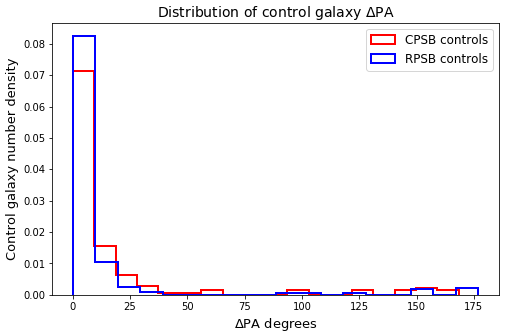
\includegraphics[width=\columnwidth]{images/JupyterPlots/Distribution-of-control-galaxy-deltaPA.png}
    \caption{Distribution of control galaxy velocity map $\Delta$PA.}
    \label{fig:controlDeltaPAs}
\end{figure}

\begin{figure}
    \centering
    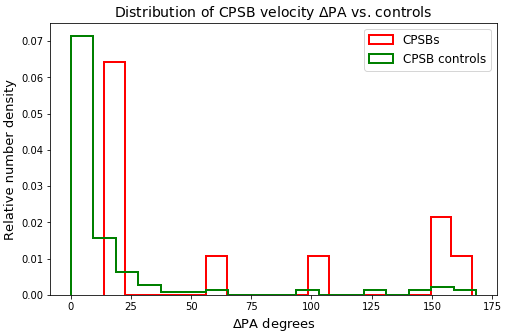
\includegraphics[width=\columnwidth]{images/JupyterPlots/Distribution-of-CPSB-dPA-vs-controls.png}
    \caption{Distribution of CPSB stellar-gas velocity $\Delta$PA vs. controls.}
    \label{fig:CPSBvsControlDeltaPAs}
\end{figure}

\begin{figure}
    \centering
    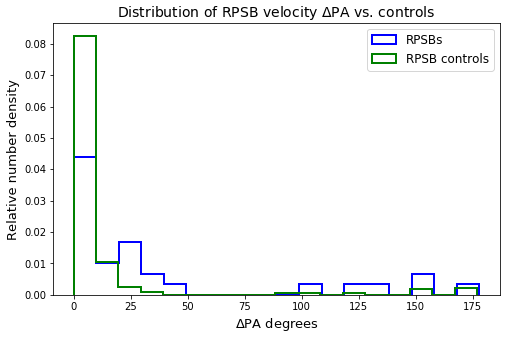
\includegraphics[width=\columnwidth]{images/JupyterPlots/Distribution-of-RPSB-dPA-vs-controls.png}
    \caption{Distribution of RPSB stellar-gas velocity $\Delta$PA vs. controls.}
    \label{fig:RPSBvsControlDeltaPAs}
\end{figure}


